\section{敏感性分析}

为检验结论的稳健性，本文将已有的方案对照与新增的参数扫描分开讨论。前者复用前文各问题的正式结果，后者仅针对问题四 4-3 的四时点滚动模型进行年度回测。

\subsection{方案对比}

表 20 汇总终端机制、滚动更新和价格信息结构的对照结果。问题二中，季节余弦终端基准叠加因果风险微调后，年度费用较固定 6000~kWh 终端基线降低 2836.86 元（0.02\%）。该变化较小，说明终端机制的主要作用是避免跨日储能透支，而非追求单日费用的显著下降。

问题三和问题四 4-3 中，全部四时点滚动相对仅 0:00 决策分别节省 351055.72 元（2.36\%）和 384819.53 元（2.44\%）。两种价格口径下的降幅接近，且 6:00 与 12:00 更新贡献绝大部分收益，故日内滚动的经济价值主要来自对负荷、光伏不确定性的及时修正。

价格完全信息下界仅将未来电价替换为实际值，负荷与光伏的信息结构、储能约束及滚动时点均保持不变；因此它衡量的是价格预测误差的经济影响，而不是所有预测变量均准确时的全局理论最优。问题 4-2 与 4-3 相对该下界的差距分别为 0.93\% 和 1.03\%，表明现有周期预测和日内门控更新已捕获大部分可用于套利的价格信息。

\Needspace{8\baselineskip}
{\footnotesize
\threelinetable{表 20\quad 模型方案与价格信息对照}{l r r r r}{%
  \textbf{对比对象} & \textbf{基准费用/元} & \textbf{对照费用或下界/元} & \textbf{费用变化/元} & \textbf{相对变化}\\
}{%
  问题二：固定终端 $\rightarrow$ 季节余弦 + 风险微调 & 14640006.24 & 14637169.37 & $-2836.86$ & $-0.02\%$\\
  问题三：仅 0:00 $\rightarrow$ 全部四时点滚动 & 14861411.71 & 14510355.99 & $-351055.72$ & $-2.36\%$\\
  问题四 4-3：仅 0:00 $\rightarrow$ 全部四时点滚动 & 15778106.07 & 15393286.54 & $-384819.53$ & $-2.44\%$\\
  问题四 4-2：现实预测 $\rightarrow$ 价格完全信息下界 & 15529514.78 & 15386096.19 & $-143418.60$ & $-0.93\%$\\
  问题四 4-3：现实预测 $\rightarrow$ 价格完全信息下界 & 15393286.54 & 15236867.28 & $-156419.25$ & $-1.03\%$\\
}
}

\subsection{参数对比}

以问题四 4-3 的正式模型为基准，取 $\rho=0.80$、场景数 $S=100$、终端软区间半宽 $h=1000$~kWh；单次仅改变一个参数，其余规则保持不变。图~\ref{fig:q4_sensitivity_cost} 与表~21 给出扫描结果；场景数各水平采用 5 个共同随机种子，误差棒为年度费用标准差。

$\rho$ 的三个离散点费用差异不超过 $0.23\%$；$S$ 从 50 至 200 时，费用由 $+0.17\%$ 变为 $-0.09\%$、单日求解时间由 1.30~s 增至 1.97~s，故保留 $S=100$；$h=500$--$1500$~kWh 时费用变化不超过 $0.02\%$。

\begin{figure}[H]
  \centering
  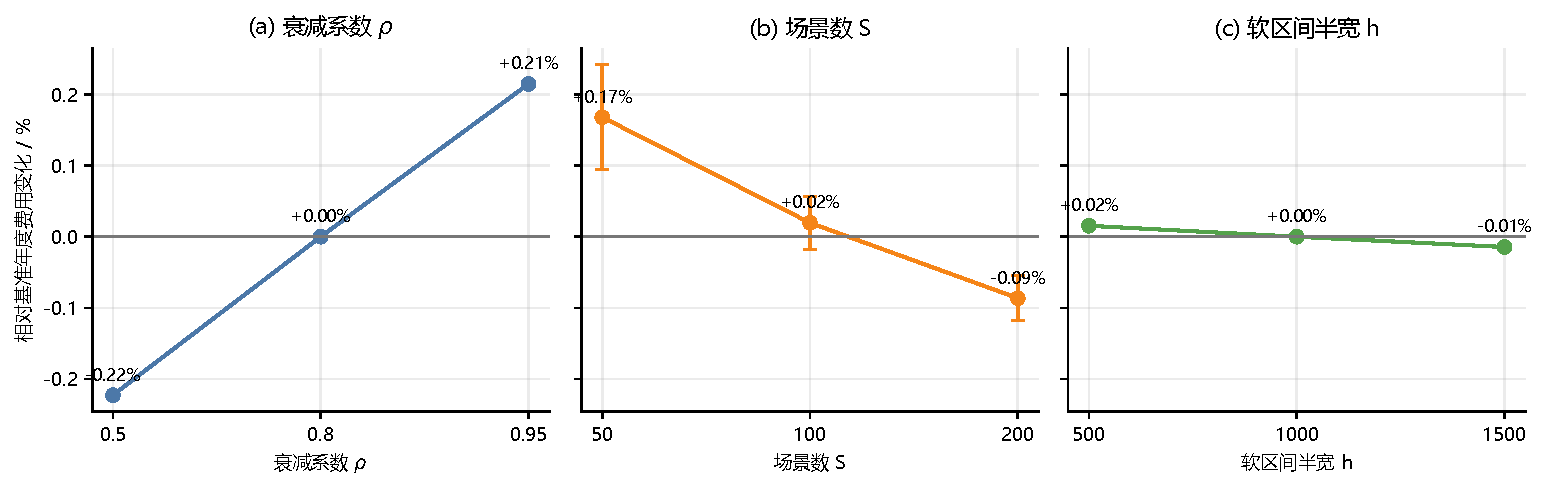
\includegraphics[width=0.60\textwidth]{../figures/问题四/问题四_4_3年度费用参数灵敏度.pdf}
  \caption{问题四 4-3 年度费用参数灵敏度}
  \label{fig:q4_sensitivity_cost}
\end{figure}

{\scriptsize\renewcommand{\arraystretch}{0.82}
\threelinetable{表 21\quad 问题四 4-3 单参数扫描结果}{l c c l}{%
  \textbf{参数} & \textbf{试验值} & \textbf{年度费用相对基准变化} & \textbf{说明}\\
}{%
  $\rho$ & 0.50 / 0.80 / 0.95 & $-0.22\%$ / $0.00\%$ / $+0.21\%$ & 三个点的差异均小于 0.23\%\\
  $S$ & 50 / 100 / 200 & $+0.17\%$ / $+0.02\%$ / $-0.09\%$ & 5 个种子均值，标准差为 0.07\% / 0.04\% / 0.03\%\\
  $h$/kWh & 500 / 1000 / 1500 & $+0.02\%$ / $0.00\%$ / $-0.01\%$ & 费用影响可忽略\\
}
}

综上，参数扰动不改变主要结论，日内滚动在两类电价口径下均带来约 2.4\% 的稳定费用节省。
